\section{Detector Layout}

\subsection{The Calorimeter (FT-Cal)}

The FT-Cal has to fulfill demanding requirements in terms of: radiation hardness, light yield, shower containment
(small radiation length and Moliere radius), fast recovery time, and good energy and time resolution.

The electron energy resolution is a crucial factor to determine precisely the photon energy and to ensure the
exclusivity of the measured reaction via the missing mass technique. However, since we are interested in low-energy
electrons and high-energy photons, the energy resolution on the latter is significantly better than the resolution on
the electron\footnote {For example, an electron energy resolution of 2\% (at 1~GeV) would result in an energy
  resolution of $\sim$0.2\% for the corresponding 10~GeV photon, allowing the use of the missing mass technique
  for most of the reactions of interest.}. The FT-Cal should have a fast recovery time ($\tau\sim$ 10~ns) to sustain
high rates with small pile-up effects and to provide the scattered electron interaction time with good accuracy
($<$1~ns) in order to reject background and to identify the relevant signals via coincidence with CLAS12. Due to the
expected high rate from electromagnetic background, the calorimeter should be highly segmented in the transverse
direction. The size of each detection element should be comparable with the characteristic transverse size of the
electromagnetic shower (Moliere radius) to contain the shower produced by incident electrons to a few readout cells,
thus minimizing rates and pile-up. Finally, the photodetectors for the light read out should work  in a sizable magnetic
field and fit within the available space. Thus, standard photomultipliers (PMTs) cannot be used while photodetectors
based on semiconductors, e.g. avalanche photodiodes (APDs), have been shown to meet the required criteria. 

To match the necessary requirements, lead tungstate (PbWO$_4$) was chosen as the scintillating material and
Large-Area APDs (LAAPDs) as the readout sensors. A similar  combination was used in the CMS-ECal~\cite{CMS-ECal},
CLAS-IC~\cite{CLAS-IC}, and PANDA-EMC~\cite{PANDA-ECal} calorimeters. Lead tungstate has a fast scintillation
decay time (6.5~ns), a small radiation length (0.9~cm), and small Moliere radius (2.1~cm). The drawback of limited
light emission (about 0.3\% of NaI(Tl)) has been mitigated by using cooled PbWO$_4$ Type-II crystals (as for the
PANDA-EMC), matched to large-area photosensors to obtain a factor of four more light per MeV of deposited energy
than the original CMS-ECal crystals.

With this design an energy resolution of the order of ($2\% /\sqrt{E\textrm{(GeV)}} \oplus 1\%$) is expected.
Other crystals, such as LSO/LYSO or the very recent LaBr, share almost all of the good specifications of
PbWO$_4$ with a light yield more than 100 times larger. However, the lack of extensive studies on radiation
hardness and the limited experience in the manufacturing procedures excluded them from consideration as an
alternative.

\begin{figure}[th!]
\centering 
\includegraphics[width=0.85\columnwidth]{fig/section.png} 
\caption{CAD drawing of the FT-Cal showing a cross section of the detector. The crystals, in purple, are enclosed in the copper thermal shield, in orange, surrounded by the insulation, in light gray. On the downstream end of the crystals (right side of the figure), the preamplifiers are shown in green. The weight of the crystals is supported by the tungsten pipe, in dark gray, which is an integral part of the beamline.}
\label{fig:ft-cal-geometry} 
\end{figure}

\subsubsection{Geometry and Coverage}

The FT-Cal is made from 332 $15\times 15\times 200$~cm$^3$ parallelepiped PbWO$_4$ Type-II crystals
arranged around the beamline with full azimuthal angular coverage ($0^\circ < \phi < 360^\circ$)  and small
forward angles acceptance ($2^\circ < \theta < 5^\circ$). The crystals are placed with their long side parallel to
the beamline to form a ring. Figure~\ref{fig:ft-cal-geometry} shows the a CAD rendering of the calorimeter. 

\subsubsection{PbWO$_4$ Crystals}

The FT-Cal PbWO$_4$ Type-II crystals were produced by the Shanghai Institute of Ceramics, Chinese Academy
(SICCAS). Since the light yield ($LY$) increases when lowering the temperature $T$ according to 
$dLY/dT \sim 3\%/^\circ$C, the calorimeter is stabilized in temperature and operated at
$T \sim 0^\circ$C. Lower temperatures were not considered due to significant complications in the
mechanical/thermal design, the reduced resistance to radiation,  and the decay time degradation of the cooled
PbWO$_4$. The length of the crystals (20~cm - corresponding to $\sim$22 radiation lengths) was chosen to
minimize the longitudinal loss and to match the available clearance.

The size of the crystal front face of 15~mm $\times$ 15~mm provides a pixelization in the transverse plane of
the PbWO$_4$ crystals consistent with the Moliere radius. All crystals were characterized using the ACCOS
(Automatic Crystal quality Control System) facility at CERN~\cite{accos}. The geometrical dimensions, as well as the
optical properties such as the longitudinal and transverse transmission and the relative light yield, were determined
for each of the crystals. Samples that were outside of the required specifications were rejected and replaced by the
manufacturer. 

The absolute $LY$ (number of detected photoelectrons per MeV deposited) was found to be $N_{pe}=220\pm 20$
at $T=0^\circ\textrm{C}\pm 0.5^\circ\textrm{C}$. For this measurement the crystal was wrapped on 5 of its faces
with 3M Vikuiti reflective film and read out by a Hamamatsu S8664-1010 LAAPD operated at a gain $G$=150
connected with optical grease on the exposed face. 

The scintillation decay time is also sensitive to the temperature. The time constant was measured using the
{\it Start-Stop} or {\it Delayed-Coincidence} method at different temperatures. As expected, an increase in the
decay constant was observed by decreasing the temperature. At $T=0^\circ\textrm{C}\pm 0.5^\circ\textrm{C}$, we
found $\tau=13.5\pm 0.6$~ns ($\tau_1=11.6\pm 0.5$~ns and $\tau_1=13.0\pm 0.2$~ns) when a single (double)
exponential form was used to fit the data.

\begin{figure}[th!]
\centering 
\includegraphics[width=0.85\columnwidth]{./fig/dk.jpeg} 
\caption{Histogram of the radiation-induced absorption coefficient, $dk$, for all SICCAS FT-Cal PbWO$_4$ crystals.}
\label{fig:dk} 
\end{figure}

The radiation hardness of the crystals was measured by irradiating them with a dose of 30~Gy of low-energy photons
using a $^{60}$Co source at the Strahlenzentrum of Giessen University~\cite{radhard}. The longitudinal transmission
was measured before and after the irradiation, calculating the variation as a function of the wavelength. The radiation
hardness of the crystals was quantified by the radiation-induced absorption coefficient defined as:

\begin{equation}
dk = \frac{1}{L}\frac{T_{bef}}{T_{irr},}
\end{equation}

\noindent
where $T_{bef}$ is the light transmission at 420~nm, the peak of the PbWO$_4$ emission spectrum, measured before
irradiation, and $T_{irr}$ is the light transmission at the same wavelength after irradiation for crystals of a given
length $L$. Crystals exhibiting greater levels of radiation damage to light transmission have higher values of $dk$.
All 332 crystals assembled in the FT-Cal were individually characterized: on average we found 
$T_{bef}$(420~nm) = $61.5 \pm 0.2$ ($\sigma=3.2$) and $T_{irr}$(420~nm) = $50.8 \pm 0.5$ ($\sigma=4.9$). 
The resulting $dk$ distribution is shown in Fig.~\ref{fig:dk}. These measurements were used to optimize the position
of each crystal in the calorimeter, placing the crystals with the highest radiation resistance, and therefore lowest
$dk$, in the areas where the highest radiation dose is expected.

\begin{figure}[th!]
\centering 
\includegraphics[width=1.0\columnwidth]{./fig/apd5.eps} 
\caption{Intrinsic gain of one APD as a function of the bias voltage and of the temperature.}
\label{fig:G-V-T} 
\end{figure}

\subsubsection{Light Readout and Electronics}
\label{sec:ftcalread}

The FT-Cal uses $10 \times 10$~mm$^2$ (model Hamamatsu S8664-1010) LAAPDs to read out the PbWO$_4$
scintillation light. APDs are very compact devices (only a few mm thick), have a large quantum efficiency at the
PbWO$_4$ light peak emission (420~nm), and  are insensitive to magnetic fields. The main disadvantage is that,
due to their low intrinsic gain ($\sim$50-200), the output signal is too small to be directly acquired, and needs to
be amplified by a suitable circuit. APDs also need to be operated at a controlled temperature to avoid variations in
gain and noise, but this does not represent a major complication since the crystals also are required to be stabilized
in temperature. Each sensor used in the FT-Cal has been characterized by measuring its gain as a function of the
applied bias voltage at a given temperature using an automated  custom facility (see Ref.~\cite{celeAPD} for more
details). The typical gain behavior $G(V_{Bias},T)$ is shown in Fig.~\ref{fig:G-V-T}. The working point (bias voltage)
was chosen in order to have the chosen gain ($G=150$) in a reasonably stable region for small variation of the biasing.
Silicon photomultiplier (SiPM) readout was not considered due to their limited dynamic range, which is not suitable for
spectroscopic applications, and the limited experience (in term of reliability, radiation hardness, stability in time, etc.)
in their use in large experiments at this time.

The APD current signal is converted to a voltage pulse that is transmitted to the subsequent electronics chain via a
trans-impedance amplifier (i.e. an amplifier that converts an input current pulse into an output voltage pulse, without
performing any time integration). This amplifier has been developed in collaboration with the Service Electronique
pour la Physique (SEP) of the Institut de Physique Nucl{\'e}aire (IPN) in Orsay. The amplifier ENC \footnote{The ENC,
  equivalent noise charge, is defined as the charge transported by an input signal giving, at the output of the amplifier,
  a signal whose amplitude is equal to the RMS of the output noise.} was measured at the operating temperature of
T=0$^\circ$C,  with ENC$\sim10400$ $e^-$ (RMS) for the nominal gain of $G=600$.  This corresponds to about 3 MeV (RMS) on the measured energy. The amplified signal is read out using the custom JLab flash
ADC VME board (a 16-channel, 12-bit, 250~MHz digitizer; referred to as the FADC250). The measurement
of the full waveform allows for the derivation of both the charge and time of the hit with the required  accuracy.

\subsubsection{Light Monitoring System}

Lead tungstate scintillating crystals are known as an appropriate material for use in total absorption shower
detectors. Unfortunately, although relatively radiation tolerant, their light output is reduced when exposed to 
radiation and recovers when the radiation source is removed. Further complications arise because at the same
irradiation intensity, changes in light output may vary from one crystal to another. In order to maintain the intrinsic
energy resolution, the crystals have to be continuously monitored and, if necessary, re-calibrated by changing the
supply voltage. The monitoring system should be able to test the response over time of the whole chain: crystal,
APD, read-out electronics. Among the different possible options (radioactive source, laser, and LED) we used an
LED-based Light Monitoring System (LMS). In spite of the need for thermal control, LEDs offer considerable
advantages: matching with crystals is simpler than for lasers, since each crystal can have a LED in front of it and
the arrangement of power lines and electrical connections is less critical than for optical fibers. The main
disadvantage is related to the complexity of the electronic circuitry: to cover a large light intensity range while
maintaining a good timing, each LED needs a separate driver, which leads for a calorimeter of significant size, to
a large number of electronic circuits.

With LEDs it is possible to obtain a shape and a duration of the monitoring-light flash that is similar to the features
of the crystal scintillation light. In fact, the emission spectrum of the monitoring light can be chosen to be similar to
the radio-luminescence spectrum of PbWO$_4$, the effective optical path length for monitoring light in the crystal
can be matched to the average path length of the scintillation light produced by an electromagnetic shower, and the
pulse length can be tuned to reproduce the PbWO$_4$ scintillation decay time. We chose a blue light LED with
wavelength close to the 430~nm emission peak of the PbWO$_4$ crystal, where radiation damage may have the
maximum effect. Each crystal is equipped with a separate LED, located on its upstream face, at the
opposite end with respect to the light sensors and electronics. The intensity can be varied in the range from 500 to
100,000 photons, pulsed at a variable rate from 62~Hz to 8~kHz, with a pulse rise time of $\sim$1~ns and a time
jitter of less than 200~ps. The system has been designed to work in the temperature range from -25$^\circ$C
to +30 $^\circ$C. The LEDs placed in the closed environment of the crystal are kept at constant temperature with an
accuracy of $\Delta T$ = 0.1$^\circ$C. The LED monitoring system is split in two boards: one containing the control
logic and the LED driver circuits, and the other, mounted in front of the FT-Cal crystals, hosting the LEDs. The two
boards are connected via a board-to-board connector that allows the required flexibility to match the FT-Cal
geometry and positioning. The LED drivers are controlled by an on-board PIC32 micro-controller accessible remotely
via Ethernet. Each LED is individually set by a programmable length and intensity pulse. The system is triggered by
an internal clock or by an external signal. In both cases the trigger signal is available for a precise time reference. 

\begin{figure}[th!]
\centering 
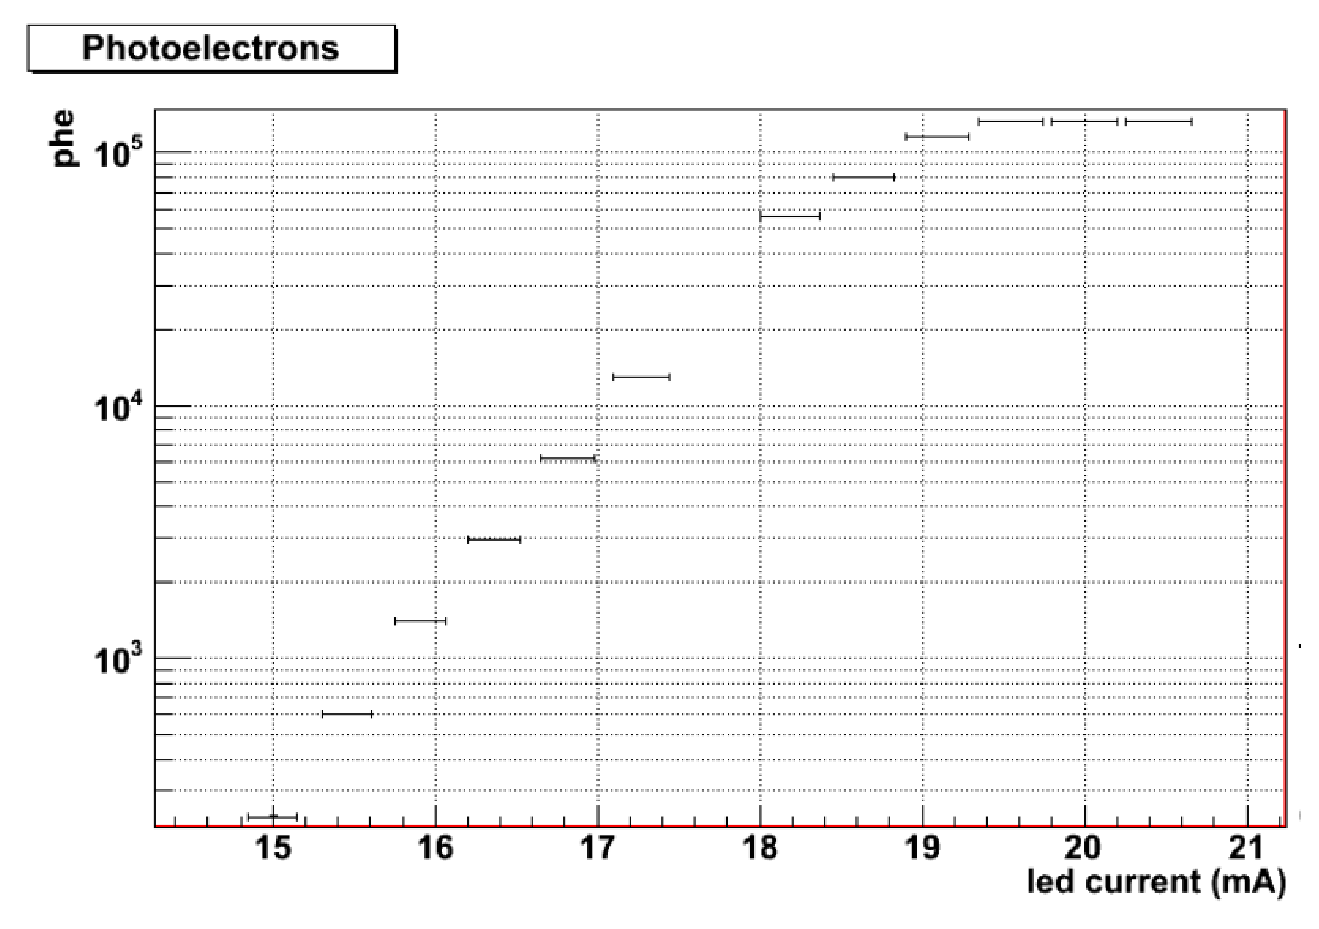
\includegraphics[width=1.0\columnwidth]{./fig/dynamics.eps}
\caption{Number of photoelectrons as a function of the LED driver current. The corresponding energy per crystal
  ranges from 10~MeV to 10~GeV.}
\label{fig:LEDperf1} 
\end{figure}

\begin{figure}[th!]
\centering 
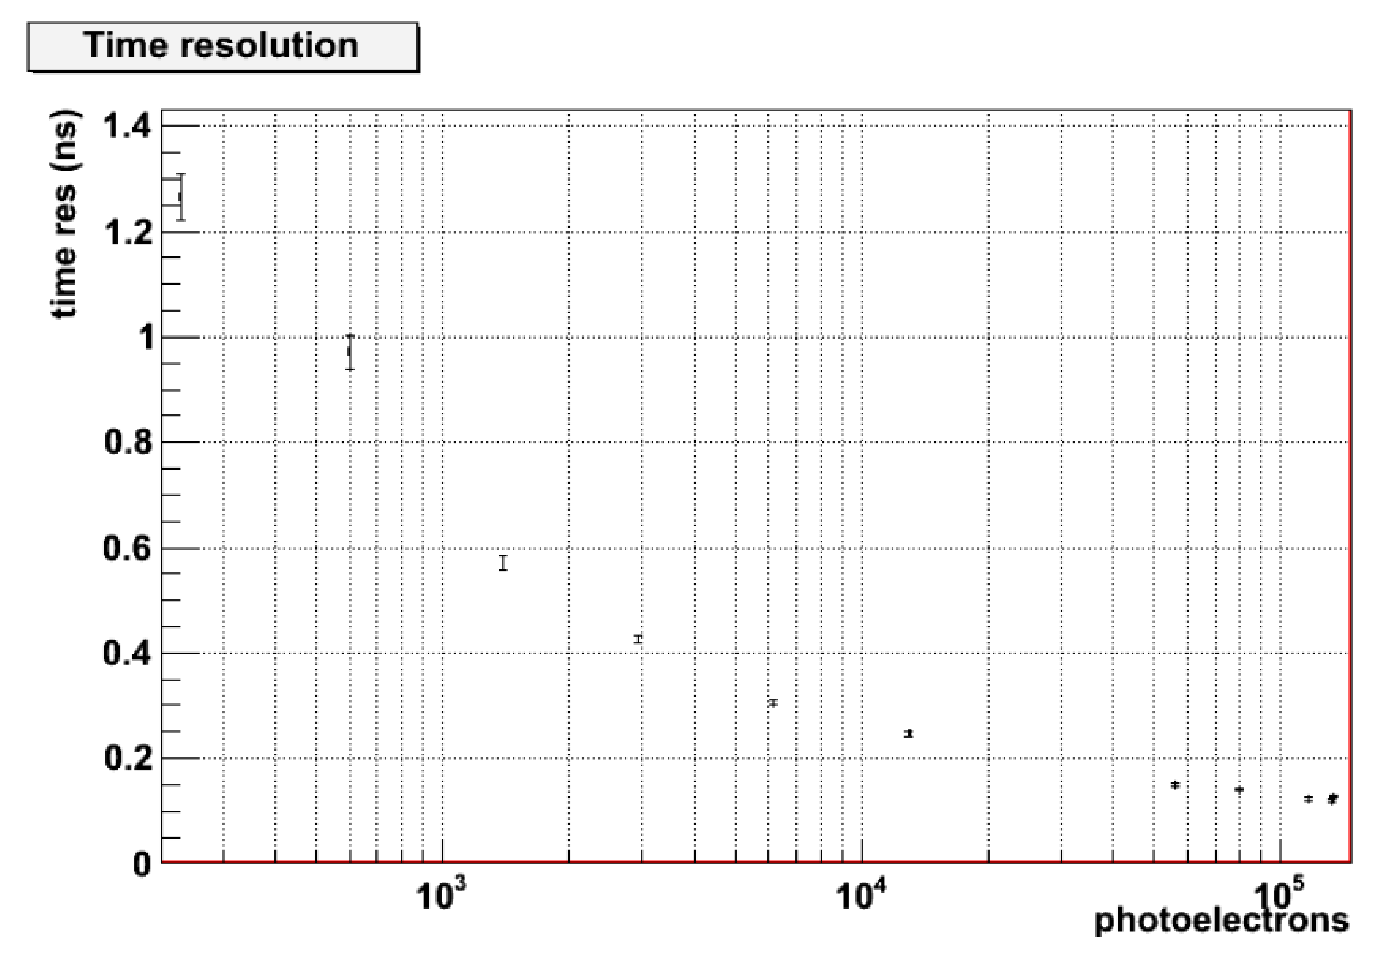
\includegraphics[width=1.0\columnwidth]{./fig/timing.eps}
\caption{Time resolution (measured as the time difference of the trigger signal and the PMT pulse) as a function of
  the LED light intensity.}
\label{fig:LEDperf2} 
\end{figure}

The performance of the LED driver has been measured by coupling a single monitoring channel to a PMT. The
performance of the system is reported in Figs.~\ref{fig:LEDperf1} and \ref{fig:LEDperf2}, where the measured
number of photoelectrons as a function of the LED current and the measured time resolution as a function of the
number of photoelectrons are shown\footnote{The time resolution is defined as the width ($\sigma$) of the time
  difference distribution between the trigger signal and the PMT output.}. Rescaling the results to take into account
the APD readout and the crystal $LY$/MeV, the equivalent energy ranges from 10~MeV (500~phe) to 10~GeV
(500k~phe) perfectly matched to the expected energy collected by each crystal. A time resolution of 100~ps is
reached at high light intensity. The long term stability of the system has been measured over a 100-hr run at
$T=+18^\circ$C. The stability of each individual channel was found to be in the range of 2\%; when the ratio of
the two channels is considered, the stability is at a level of a few parts per thousand.

\subsubsection{Slow Controls and Interlocks}

The FT-Cal slow controls are part of the CLAS12 EPICS system~\cite{daq}. The APDs need to be reverse-biased
with a positive high-voltage power source. The APD intrinsic gain depends on the bias voltage with
$\frac{1}{G}\frac{\Delta G}{\Delta V} \sim4 \%$ and, therefore, the power supply needs to be stable in time, with
low output noise. We chose the CAEN A1520P board designed for the CMS electromagnetic calorimeter. The power
supply fulfills  all our requirements in terms of dynamic range, linearity, and noise. Each board is equipped with 12
independent channels that each control a group of ten APDs with relative gain variations not greater than 3\%.

The amplifiers used in the FT-Cal need to be operated with +5~V and -5~V. The power consumption from each of the
two voltage sources is approximately 70~mW, almost independent of the event rate, giving a power consumption of
$\sim$140~mW per board, for a total of 56~W for a 400-channel calorimeter. The full FT-Cal is powered by a
Wiener MPOD MPV8008L power supply. Sensing feedback is implemented to compensate the voltage drop across the
connecting cables.

Temperature regulation is provided by a Lauda XT150 chiller unit. This is a self-regulating unit and does not require
external feedback, however, the settings and monitored parameters are sent to EPICS for recording via a
{\it streamDevice} module. The FT-Cal temperature is monitored by a set of PT100 thermoresistors located at
different positions within the crystal assembly and read by a {\it cRio} module, which is part of the interlock system.
The flow of nitrogen gas, which is purged in the preamplifier area to prevent moisture build-up at low temperature,
is measured with a flowmeter and monitored by the same {\it cRio} system. The latter is also used to read the output
of two humidity sensors located in the preamplifier area. 

The {\it cRio} system is the main component of the interlock system that was designed to provide a fast shutdown
mechanism for all critical components in case abnormal conditions are detected. The parameters that are monitored
are the FT-Cal temperatures, the nitrogen flow, and the humidity. If any of the measured values is found to be
outside user-defined ranges, the system disables the FT-Cal high voltage (HV) and low voltage (LV) crates and stops
the chiller to prevent any damage to the detector or surrounding elements.

\subsubsection{Mechanical Design}

The mechanical design of the calorimeter is driven by three considerations: minimization of the empty spaces between
crystals, cooling to $0^\circ$C, and optimal coverage of the required acceptance without interference with the rest
of CLAS12.

\begin{figure}[th!]
\centering 

\includegraphics[width=1.0\columnwidth]{./fig/sc-assembly.eps}
\caption{Single crystal assembly: from the left (front) to the right (back), the PEEK support that holds the nose with
  the LED housing, the crystal wrapped in 3M Vikuiti reflective film, the LAAPD in the PEEK housing, and the
  preamplifier.}
\label{fig:crystalassembly} 
\end{figure}

The building blocks of the calorimeter are the individual lead-tungstate crystals. Each crystal is
$15\times 15\times200$~mm$^3$, for a weight of 370~g. Each crystal is optically coupled to a LAAPD on its
back face and to an LMS LED on its front face for calibration. To achieve the maximum light collection efficiency,
the APD covers almost the entire area of the downstream end of the crystal, so the LED for monitoring has to be
mounted on the upstream end. This reflects onto the mechanical design of the single crystal assembly as a monolithic
self-supporting element made of the crystal itself, the APD, the reflective wrapping, and the crystal support
structure. To avoid dead volume in the detector, the mechanical support for each crystal is provided only by the
wrapping. We chose 3M Vikuiti reflective film. This material is non-conductive, has a reflectivity higher than
aluminized Mylar and, if properly heat-formed, can hold the weight of a crystal. The reflective film is glued on the
sides of a pair of front/back PEEK custom-machined blocks that hold the LAAPD and the LED, respectively.
Figure~\ref{fig:crystalassembly} shows a CAD rendering of the single crystal assembly from the front PEEK
support to the preamplifier.

\begin{figure}[th!]
\centering 
\includegraphics[width=1.0\columnwidth]{./fig/raff.jpeg}
\caption{The copper thermal/grounding shield for the FT-Cal. The right figure shows the ensemble of the copper shield with the cooling pipes shown in blue. These are located on the back plate, on the outer cylinder and on the inner shield.  The left figure shows the cooling pipe circuit inside the inner shield. FIGURE WILL BE REPLACED WITH NEW ONE AND THE CAPTION UPDATED}
\label{fig:piping} 
\end{figure}

The crystal assemblies are installed in a matrix to provide complete shower containment for electrons in the FT-Cal
angular acceptance. Two copper plates, placed in front of and on the back of the crystals, define the positioning for
the crystal assemblies. On the APD side, the preamplifiers, one for each crystal, are connected to the readout
motherboard, which is designed to provide power distribution and signal collection for each channel. The mechanical
structure allows for the replacement of individual preamplifiers if needed. The front and back copper plates are
connected by a copper cylinder on the outside and by an inner copper shield to form a closed vessel that surrounds
the crystal matrix to provide proper grounding and the required thermal stability and uniformity. Cooling is provided
by 5-mm diameter copper pipes installed on the outside of the vessel as shown in Fig.~\ref{fig:piping}. 

The FT calorimeter has been designed to operate between 0$^\circ$C and room temperature. The FT-Cal cooling is
achieved via circulation of coolant in the circuit attached to the rear copper plate and on the inner and outer copper
vessels. The cooling system was designed to compensate the heat load in the region surrounding the FT, taking into
account 20~mm of insulating foam (polyisocianurate thermal conductivity 0.024~W/mK) and from the amplifiers, which
dissipate $\sim$50~W. The insulation is less effective between the calorimeter and the inner tungsten pipe that
holds the entire FT (see Section~\ref{sec:integration}) because of the limited space for the insulation and the
presence of the support structures that bring the overall thermal conductance in that region to 0.056~W/mK.

During the design phase, Finite Element Analysis calculations were performed to optimize the cooling circuit and the
insulation parameters in order to reach the design temperature and uniformity. These studies indicated that the
coldest part of the external calorimeter enclosure is the tungsten cone that is expected to stabilize at a temperature
just above the dew point. Measurements performed after the calorimeter assembly confirmed these results.

\subsection{The Hodoscope (FT-Hodo)}

The primary aim of the FT-Hodo is to discriminate between photons and electrons that produce the electromagnetic
shower in the calorimeter. Specifically, electrons are identified by hits in the hodoscope array that are correlated
in both position and time with a cluster observed in the calorimeter. The FT-Hodo is comprised by an array of 232 plastic
scintillator (Eljen-204) tiles segmented in two layers to suppress contributions from the splash-back of the
electromagnetic shower created by events depositing energy in the FT-Cal. The scintillators provide fast timing and
sufficient resistance to radiation damage for use in the high-rate and high-dose environment of the FT. The geometry
and readout of the hodoscope are constrained by the surrounding apparatus. Specifically, the device is positioned
upstream of the FT-Cal, fitting into a circular disk of diameter 330~mm and 42~mm depth. The readout is achieved
using $3 \times 3$~mm$^2$ Hamamatsu S13360-3075PE SiPMs (50\% photon detection efficiency for 450~nm
photons) coupled to 5-m-long clear optical fibers (Kuraray clear-PSM with attenuation length $>10$~m), which are
fusion spliced to $\sim$30~cm long wavelength shifting (WLS) Kuraray Y11 fibers (attenuation length of $> 3.5$~m),
embedded in the scintillator tiles. The splicing induces a photon loss of less than 2\%, where the use of optical fibers
allows the captured light to be transported with a light loss of less than $\sim$40\% over the 5~m path to the SiPM.
This readout design of the FT-Hodo addresses the need to minimize material in the detector acceptance, to operate
in regions of high magnetic fields produced by the CLAS12 solenoid and torus magnets, and to tolerate the high
background radiation environment. 

Each layer of the FT-Hodo is comprised of 44 15~mm$\times$15~mm (P15) and 72 30~mm$\times$30~mm (P30)
scintillators arranged as shown in Fig.~\ref{Fig:FTHodoLayout}. The upstream and downstream layers utilize 7-mm
and 15-mm thick scintillator tiles, respectively. The upstream (thin) layer is employed to reduce photon conversion in
the FT-Hodo, while the thicker layer provides the signal with the most accurate timing information for the event. To
increase the number of scintillation photons collected from each tile, four WLS fibers were embedded in the P30
tiles and 2 in the P15 tiles. In addition, the WLS fibers were glued with Bicron BC-600 glue (CHECK Epotek 301-2)
inside diagonal holes to maximize the path length in the scintillator and to allow for the tiles to be arranged without
any dead space between the elements. Each tile was polished and painted with two layers of Bicron BC-620 reflective
paint for the sides and 3 layers for the scintillator faces and secured in position on the surface of a 2-mm-thick
plastic support board. There is a 9~mm clearance for each layer for routing the optical fibers to the readout
electronics through a $\Delta$-shaped sheathing on the bottom end of the FT-Hodo. The front and back faces are
covered by light-proof carbon fiber material that is screwed onto supporting structures made out of hexagonal
plastic spacers (15-mm wide and 22- or 15-mm tall depending on the layer). This results in a total detector thickness
of 44~mm. A 1-mm thick plastic strip traces the outer contour of the FT-Hodo and is glued on the spacer supports.
Figure~\ref{Fig:CADFT-Hodo} shows a CAD drawing of the FT-Hodo showing half of one layer of tiles, the location
of the plastic supports for the light-proofing structure, and the plastic strip.  

\begin{figure}[th!]
\centering 
\includegraphics[width=0.85\columnwidth]{./fig/FTHodoLayout.pdf} 
\caption{The arrangement of plastic scintillator tiles in the FT-Hodo. The blue (red) squares represent the
  15~mm$\times$15~mm (30~mm$\times$30~mm) tiles for each layer.} 
\label{Fig:FTHodoLayout} 
\end{figure}

\begin{figure}[th!]
\centering 
\includegraphics[width=0.85\columnwidth]{./fig/CADFT-Hodo.pdf} 
\caption{CAD drawing of the FT-Hodo showing one layer, the location of the plastic spacers, and the plastic
  strip that traces the outer contour. } 
\label{Fig:CADFT-Hodo} 
\end{figure}

With the typical maximum radiation doses determined through Geant4 simulations with realistic beam and target
parameters, and without the shielding effects of the M{\o}ller cone (see Section~\ref{sec:integration}), the
FT-Hodo will experience a light loss of 20\% in the WLS fibers after 3.5 years, whereas the plastic scintillators will
experience a light loss of 20\% after 300~years~\cite{ft-tdr}. Both scintillators and fibers also show natural
annealing processes, which can effectively compensate for the radiation damage~\cite{ft-tdr}.  

The analog signal from the SiPM is fed directly to a custom-designed preamplifier board designed by the
INFN-Genova Electronics Group. The boards host 8 independent channels each coupled to a SiPM and are mounted
in pairs in the slots of a custom crate, mechanically compatible with the VME standard. The 16 SiPMs connected to
each pair of boards are mounted on a mezzanine printed circuit board, which distributes the bias HV to each SiPM
and collects their signals for the amplifier inputs. The schematic of one channel of the SiPM amplifier board,
excluding the HV bias network is shown in Fig.~\ref{Fig:FTHODOAmpBoard}. The first stage is based on a bipolar
junction NPN transistor in a common base configuration, while the second is composed by a OPA694 operational
amplifier in a non-inverting configuration. The two BRF92 transistors have been chosen since they are low-noise
transistors with a high cut-off frequency and good stability. The two stages are coupled together with a 100~nF
capacitor to remove the DC component of the signal from the second transistor. The amplifier is coupled to the
output connector through a 100~nF capacitor and a 50~$\Omega$ resistor to remove any DC component from the
last stage and to match the impedance of the output cable. 

\begin{figure}[th!]
\centering 
\includegraphics[width=1.0\columnwidth]{./fig/FTHODOAmpBoard.pdf} 
\caption{Schematic of a single channel of the amplifier board for the SiPM.} 
\label{Fig:FTHODOAmpBoard} 
\end{figure}

The signal from each SiPM after amplification is continuously digitized by the JLab FADC250 boards and, if the
trigger condition is satisfied, samples are stored for further analysis. The data acquisition and slow controls system
for the FT-Hodo are similar to the FT-Cal (see Section~\ref{sec:ftcalread} for more details). The SiPMs operate
with a bias voltage of 50-55.5~V, which is provided by three CAEN A1737P HV boards. 30 independent HV channels
are used to operate each SiPM board that hosts 8 sensors. These groups of 8 SiPMs were selected according to their
gain. The HV distribution to the groups of 8 SiPMs is implemented on the mezzanine boards that also hosts a
compensation circuit to allow for the independent regulation of each SiPM bias voltage up to a maximum of 0.4~V. The
low voltage system used for the FT-Hodo is the same as the one used for FT-Cal. Controls of both the HV
and LV for the detector are provided by the CLAS12 EPICS slow controls system~\cite{daq}. Similarly to the FT-Cal,
the status of the critical components, in this case the temperature of the preamplifier crate, is incorporated into
the interlock system that is programmed to disable the HV and LV crates if abnormal conditions are detected.

\subsection{The Micromegas Tracker (FT-Trk)}

For a precise determination of the scattered electron angle, a tracker complements the FT-Cal and FT-Hodo
detectors. The FT-Trk uses the same technology adopted by the CLAS12 central and forward Micromegas detectors.
We refer to Ref.~\cite{mm} for a detailed description of  these devices. In this section we describe the specific
design of the FT-Trk.

\begin{figure}[th!]
\centering 
\includegraphics[width=1.0\columnwidth]{./fig/fttrk_layout.png}
\caption{3D view of the upstream face of the FT-Trk Micromegas tracker equipped with front-end electronics.}
\label{fig:ft-trck} 
\end{figure}

Two double-layers of Micromegas detectors are located in front of the hodoscope, in the space between the FT
and the High Threshold Cherenkov Counter (HTCC)~\cite{htcc}. The two detectors are indeed a good compromise
to achieve an efficient background rejection and track reconstruction with a low material budget. Each layer is
composed of a double-faced Micromegas disk built on a common printed circuit board (PCB). Each side of the PCB
displays strips, the downstream strips being perpendicularly oriented to the upstream strips. This particular geometry
enables the determination of the $(x,y)$ coordinates (perpendicular to the beam $z$-axis) of a track. To limit the
number of electronics channels, the pitch chosen was 500~$\mu$m, which leads to a resolution better than
$500/\sqrt{12} \sim 150$~$\mu$m. A drift space of 5~mm, together with an amplification gap of 128~$\mu$m,
provides good efficiency. The two double-layers, centered on the beam axis, cover polar angles from 2.5$^\circ$ to
4.5$^\circ$ with an active area defined between a 70~mm inner radius and a 143~mm outer radius. The total number of
channels is 3072. Figure~\ref{fig:ft-trck} shows the CAD implementation of the detector. The FT-Trk readout uses
the same data acquisition scheme adopted for the CLAS12 Barrel Micromegas Tracker (BMT)~\cite{mm}, which consists of
a Front-End Unit (FEU) and a Back-End Unit (BEU). 

The front-end electronics are responsible for signal preamplification, shaping, buffering during the trigger generation
process, data digitization, and compression. Due to the limited space available, the front-end electronics are designed
to be placed off-detector. Micro-coaxial cable assemblies connect the detectors and the front-end boards. The
non-amplified analog signals transit via the cable assemblies from the chambers to the front-end electronics. The
512-channel FEUs are housed in 4U crates attached to the FT-Cal mechanical supports and  located in the shadow of
the CLAS12 torus coils. The back-end electronics are responsible for data concentration, providing the interface to
the CLAS12 event building system and are the same units used for the BMT~\cite{mm}.

Each Micromegas layer is powered with 450~V for the micro-mesh and 1000~V for the drift electrode. The FT-Trk
front-end power supply is located 12~m away from the crates. The 15~W power produced by each crate is dissipated by
compressed air. An interlock system between the cooling infrastructure and the low voltage power supply prevents
powering the front-end crates when cooling is off. 

The gas used is a mixture of argon, isobutane (up to 10\%), and CF$_4$ (up to 5\%). The use of CF$_4$ ensures 
good time resolution (around 10-15~ns). The gas distribution system is the same one used by the BMT.
